\section{Utilisation du logiciel}
\subsection{Fonctionnement global}

\begin{figure}[!ht]
\begin{center}
        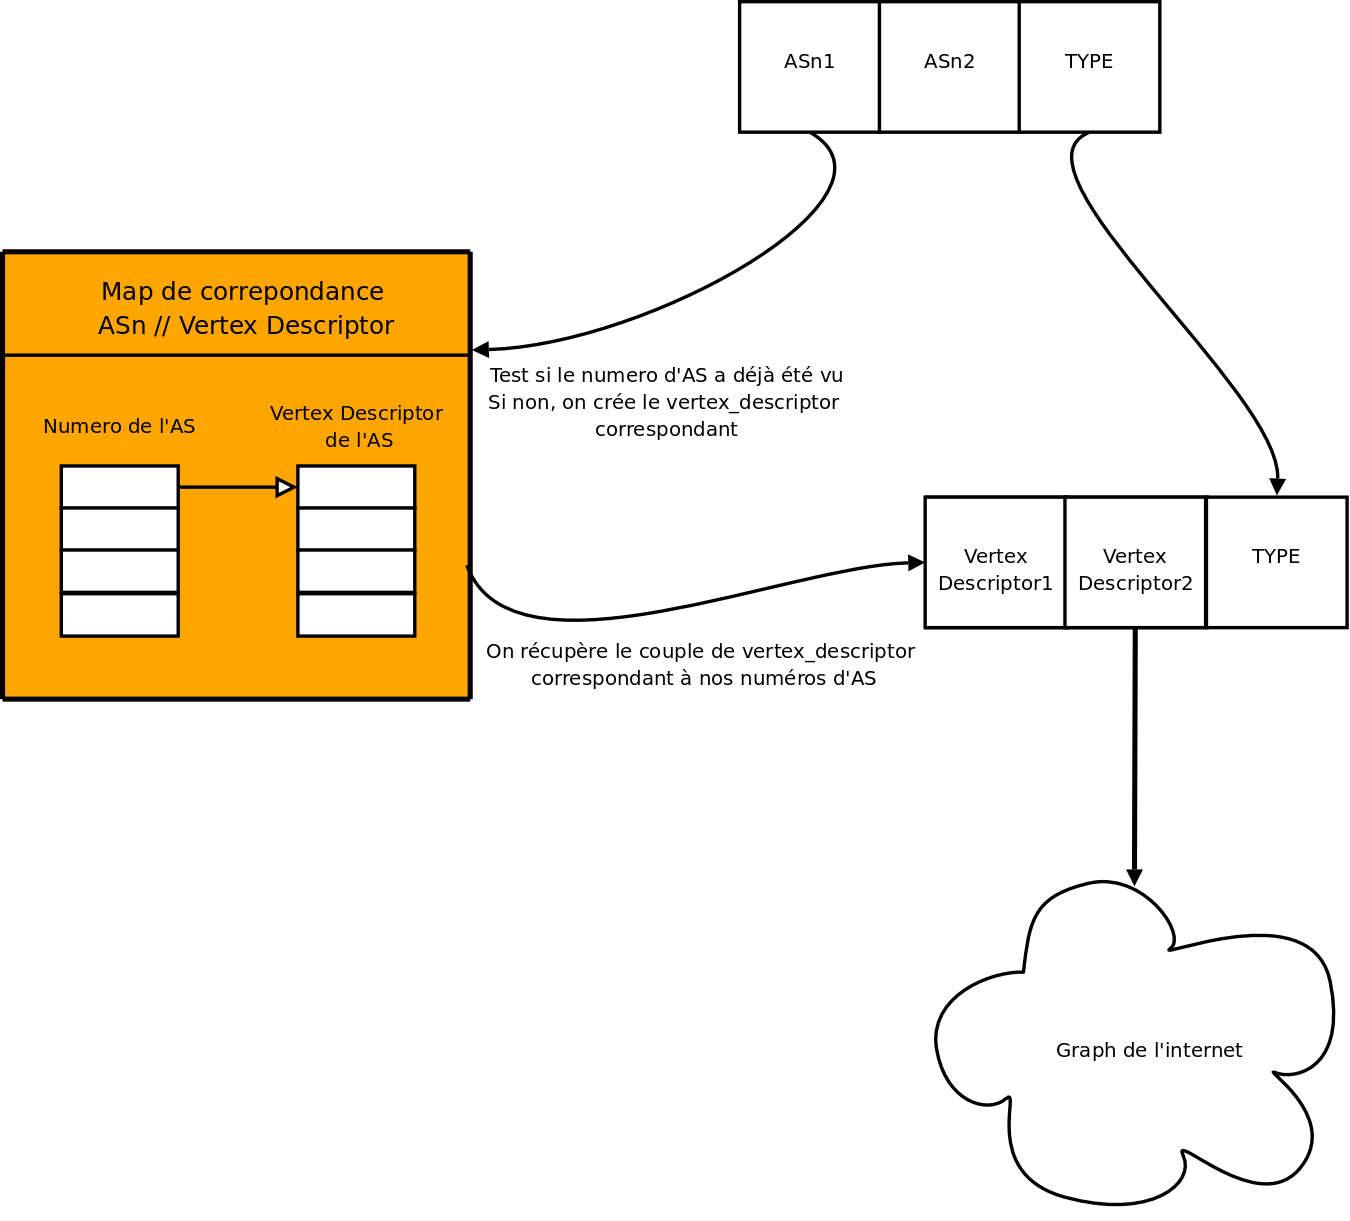
\includegraphics[width=0.7\textwidth]{./schema/file_parser.png}
\caption{Le fonctionnement du file\_parser (EVOR dit : ``Sch\'ema useless'' }
\label{file_parser}
\end{center}
\end{figure}


ATTENTION : \'ebauche pour cette partie.
\subsection{Description du programme}

Le programme tel que le voit l'utilisateur est une fen\^etre graphique avec un menu en haut, une zone d'affichage au centre, et une zone de notification en bas.

\begin{figure}[ht]
\centering
 \fbox
 {
 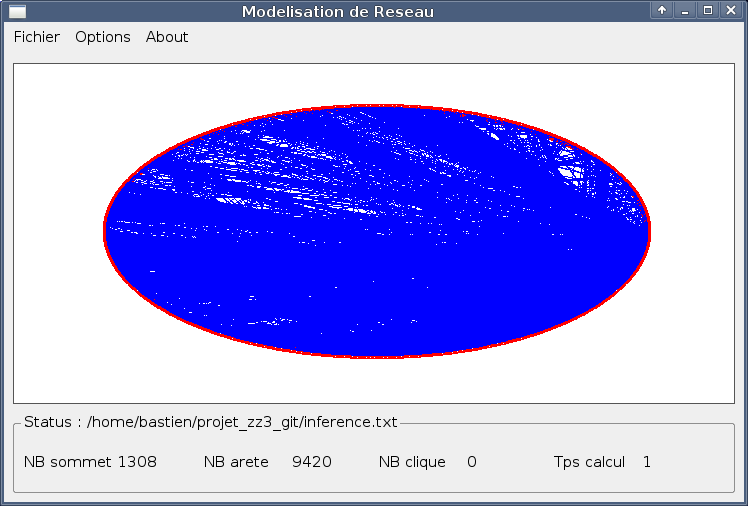
\includegraphics[width=16cm]{./schema/capture_ecran_programme.png}
 }
  \caption{\label{ecran_principal}Ecran principal du programme}
\end{figure}


Le menu comporte trois types d'entr\'ees :
\begin{description}
 \item[Fichier] permet l'ouverture des fichiers de donn\'ees \`a lire ou la fermeture du programme,
 \item[Options] permet les interactions avec le graphe telles que l'effacement de la zone d'affichage ou encore les recherche d'informations sur un AS,
 \item[About] permet l'affichage d'informations sur le programme.
\end{description}


